\documentclass[12pt,a4paper]{article}
\usepackage[utf8]{inputenc}
\usepackage[margin=1in]{geometry}
\usepackage{amsmath}
\usepackage{graphicx}
\usepackage{listings}
\usepackage{xcolor}
\usepackage{tikz}
\usetikzlibrary{shapes.geometric, arrows, positioning}
\usepackage{hyperref}

% Code listing style
\lstset{
    language=C++,
    basicstyle=\ttfamily\small,
    keywordstyle=\color{blue}\bfseries,
    commentstyle=\color{gray}\itshape,
    stringstyle=\color{red},
    numbers=left,
    numberstyle=\tiny\color{gray},
    stepnumber=1,
    numbersep=8pt,
    backgroundcolor=\color{white},
    showspaces=false,
    showstringspaces=false,
    showtabs=false,
    frame=single,
    tabsize=4,
    captionpos=b,
    breaklines=true,
    breakatwhitespace=false,
    escapeinside={(*@}{@*)},
}

\title{\textbf{Implementing Fully Non-Blocking CGI}}
\author{Web Server Architecture Guide}
\date{\today}

\begin{document}

\maketitle

\begin{abstract}
This document presents a comprehensive approach to implementing a fully non-blocking Common Gateway Interface (CGI) execution system in a high-performance web server. We discuss the architecture, event loop integration, process management, and asynchronous I/O patterns required to handle CGI requests without blocking the server's main event loop.
\end{abstract}

\tableofcontents
\newpage

\section{Introduction}

\subsection{The Blocking Problem}

Traditional CGI implementations suffer from several blocking operations:
\begin{itemize}
    \item \textbf{Process Creation}: Forking and executing CGI scripts
    \item \textbf{I/O Operations}: Writing request body to CGI stdin
    \item \textbf{Process Wait}: Waiting for CGI process termination
    \item \textbf{Response Reading}: Reading CGI output from stdout
\end{itemize}

In a single-threaded event-driven server, any blocking operation prevents the server from handling other clients, severely degrading performance and scalability.

\subsection{Solution Overview}

The solution involves:
\begin{enumerate}
    \item Using \texttt{socketpair()} for bidirectional non-blocking communication
    \item Integrating CGI file descriptors into the main event loop
    \item Non-blocking process monitoring with \texttt{waitpid(WNOHANG)}
    \item Asynchronous request body writing and response reading
\end{enumerate}

\section{Architecture Overview}

\subsection{Component Structure}

The non-blocking CGI system consists of three main components:

\begin{figure}[h]
\centering
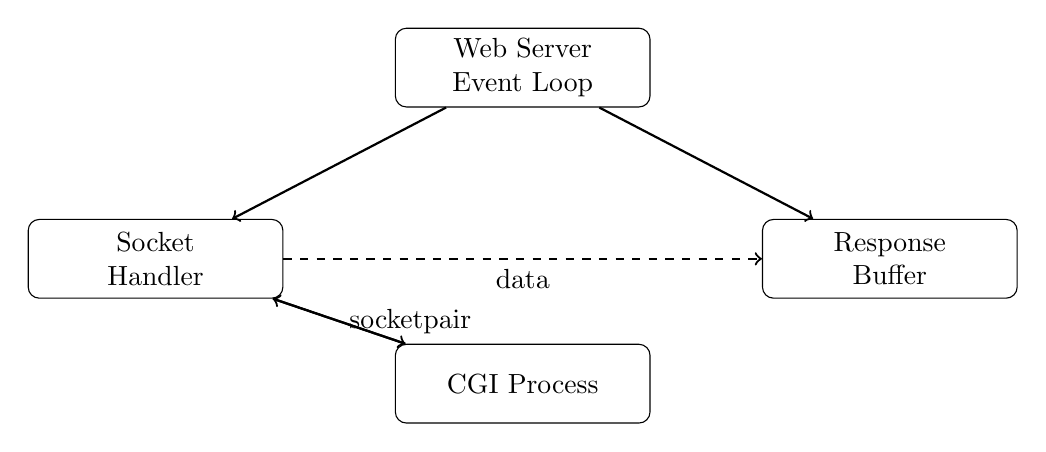
\begin{tikzpicture}[
    node distance=2cm,
    box/.style={rectangle, draw, text width=3cm, text centered, rounded corners, minimum height=1cm},
    arrow/.style={->, thick}
]
    \node[box] (server) {Web Server\\Event Loop};
    \node[box, below left=of server] (stream) {Socket\\Handler};
    \node[box, below right=of server] (response) {Response\\Buffer};
    \node[box, below=3cm of server] (cgi) {CGI Process};
    
    \draw[arrow] (server) -- (stream);
    \draw[arrow] (server) -- (response);
    \draw[arrow] (stream) -- (cgi) node[midway, right] {socketpair};
    \draw[arrow] (cgi) -- (stream);
    \draw[arrow, dashed] (stream) -- (response) node[midway, below] {data};
\end{tikzpicture}
\caption{CGI Non-Blocking Architecture}
\end{figure}

\begin{itemize}
    \item \textbf{Socket Handler}: Handles I/O events for the CGI socketpair
    \item \textbf{Response Buffer}: Buffers CGI output and manages response state
    \item \textbf{Process Monitor}: Tracks CGI process and handles termination
\end{itemize}

\section{Socket Pair Creation and Setup}

\subsection{Why Socketpair?}

The \texttt{socketpair()} system call creates a bidirectional communication channel, superior to traditional pipe-based approaches:

\begin{itemize}
    \item \textbf{Bidirectional}: Single descriptor for both read and write
    \item \textbf{Full-Duplex}: Simultaneous reading and writing
    \item \textbf{Socket Semantics}: Compatible with event loops (epoll/kqueue)
    \item \textbf{Non-Blocking}: Easily set to O\_NONBLOCK mode
\end{itemize}

\subsection{Setup Process}

\begin{lstlisting}[caption=Socketpair Creation]
int sv[2];  // Socket pair array

// Create bidirectional Unix domain socket pair
socketpair(AF_UNIX, SOCK_STREAM, 0, sv);

// Fork CGI process
pid_t pid = fork();

if (pid == 0) {
    // Child process (CGI)
    close(sv[0]);           // Close parent's end
    dup2(sv[1], STDIN_FILENO);   // Redirect stdin
    dup2(sv[1], STDOUT_FILENO);  // Redirect stdout
    close(sv[1]);
    
    // Execute CGI script
    execve(script_path, args, envp);
    exit(1);
}

// Parent process (web server)
close(sv[1]);  // Close child's end

// Set non-blocking mode
fcntl(sv[0], F_SETFL, O_NONBLOCK);

// sv[0] is now ready for event loop
return sv[0];
\end{lstlisting}

\subsection{Key Advantages}

\begin{enumerate}
    \item \textbf{Single FD}: Only one file descriptor to monitor
    \item \textbf{Efficiency}: No need for separate pipes for stdin/stdout
    \item \textbf{Simplicity}: Unified I/O handling logic
\end{enumerate}

\section{Event Loop Integration}

\subsection{The Event Loop Pattern}

Modern high-performance servers use event-driven I/O multiplexing:
\begin{itemize}
    \item \textbf{Linux}: epoll (edge or level-triggered)
    \item \textbf{BSD/macOS}: kqueue
    \item \textbf{Portable}: select/poll (legacy)
\end{itemize}

\subsection{Adding CGI Socket to Event Loop}

The CGI socketpair must be registered for monitoring:

\begin{lstlisting}[caption=Event Loop Registration]
// After socketpair creation
int cgi_fd = sv[0];  // Parent's end
pid_t cgi_pid = pid;

// Create handler for this CGI connection
CGIHandler* handler = create_cgi_handler(cgi_fd, cgi_pid);

// Register for READ and WRITE events
// READ: Monitor CGI output
// WRITE: Send request body when socket is writable
int events = EVENT_READ;
if (has_request_body)
    events |= EVENT_WRITE;

add_to_event_loop(cgi_fd, events, handler);

// Register process for monitoring
register_child_process(cgi_pid, handler);
\end{lstlisting}

\subsection{Event Types}

\begin{table}[h]
\centering
\begin{tabular}{|l|p{8cm}|}
\hline
\textbf{Event} & \textbf{Purpose} \\
\hline
READ & CGI has written data to stdout (available to read) \\
\hline
WRITE & Socket ready to accept more data (can write request body) \\
\hline
ERROR & Socket error occurred \\
\hline
HUP/CLOSE & CGI closed its end of the socket \\
\hline
\end{tabular}
\caption{Event Types for CGI Socket}
\end{table}

\section{Non-Blocking Process Management}

\subsection{The waitpid() Problem}

Traditional \texttt{waitpid()} blocks until a child process terminates, which is unacceptable in an event-driven server.

\subsection{Non-Blocking Solution}

Use \texttt{waitpid()} with \texttt{WNOHANG} flag:

\begin{lstlisting}[caption=Non-Blocking Process Monitoring]
void check_child_processes() {
    pid_t pid;
    int status;
    
    // WNOHANG: Return immediately if no child has exited
    while ((pid = waitpid(-1, &status, WNOHANG)) > 0) {
        // Process has exited
        if (WIFEXITED(status)) {
            // Normal termination
            int exit_code = WEXITSTATUS(status);
        } else if (WIFSIGNALED(status)) {
            // Terminated by signal
            int signal = WTERMSIG(status);
        }
        
        // Find corresponding handler
        CGIHandler* handler = find_handler_by_pid(pid);
        if (handler) {
            notify_process_exit(handler, status);
        }
    }
}
\end{lstlisting}

\subsection{Integration Strategy}

Call \texttt{check\_child\_processes()} periodically:
\begin{itemize}
    \item \textbf{After each event loop iteration}: Minimal latency
    \item \textbf{Using SIGCHLD handler}: More efficient (set flag, check in loop)
    \item \textbf{Timeout-based}: Check every N milliseconds
\end{itemize}

\subsection{Handler Notification}

When a CGI process exits:
\begin{enumerate}
    \item \texttt{waitpid()} returns the PID
    \item Lookup corresponding handler via PID
    \item Notify handler of process exit
    \item Mark response as EOF (no more data coming)
    \item Server completes sending buffered data
    \item Clean up resources (close FDs, free memory)
\end{enumerate}

\section{Asynchronous Request Body Writing}

\subsection{Challenge}

For POST/PUT requests, the request body must be sent to CGI's stdin. This can be:
\begin{itemize}
    \item Small (in-memory buffer)
    \item Large (temporary file on disk)
\end{itemize}

Synchronous writing blocks the server; solution is asynchronous writes.

\subsection{Write State Management}

Track writing progress:
\begin{itemize}
    \item \textbf{Body Source}: In-memory string or file descriptor
    \item \textbf{Write Offset}: Bytes already written
    \item \textbf{Remaining}: Bytes left to write
\end{itemize}

\begin{lstlisting}[caption=Request Body State]
struct CGIWriteState {
    char* body_buffer;        // In-memory body
    size_t buffer_size;       // Size of buffer
    char* temp_file_path;     // Path to temp file
    int temp_file_fd;         // Open FD for reading
    size_t bytes_written;     // Progress tracker
};
\end{lstlisting}

\subsection{Write Algorithm}

\begin{lstlisting}[caption=Asynchronous Body Writing]
int handle_write_event(int cgi_fd, struct CGIWriteState* state) {
    if (state->bytes_written >= state->buffer_size && state->temp_file_fd == -1)
        return EVENT_CONTINUE;
    
    if (state->temp_file_fd != -1) {
        // Read chunk from temp file
        char buffer[4096];
        ssize_t nread = read(state->temp_file_fd, buffer, sizeof(buffer));
        
        if (nread <= 0) {
            // EOF or error: done writing
            close(state->temp_file_fd);
            state->temp_file_fd = -1;
            remove_event_flag(cgi_fd, EVENT_WRITE);
            return EVENT_CONTINUE;
        }
        
        // Write to CGI
        ssize_t nwritten = write(cgi_fd, buffer, nread);
        
        if (nwritten < 0) {
            if (errno == EAGAIN || errno == EWOULDBLOCK)
                return EVENT_CONTINUE;  // Try again later
            return EVENT_ERROR;
        }
        
        // Partial write: seek back
        if (nwritten < nread) {
            lseek(state->temp_file_fd, -(nread - nwritten), SEEK_CUR);
        }
    } else {
        // Write from in-memory buffer
        const char* data = state->body_buffer + state->bytes_written;
        size_t remaining = state->buffer_size - state->bytes_written;
        
        ssize_t nwritten = write(cgi_fd, data, remaining);
        
        if (nwritten < 0) {
            if (errno == EAGAIN || errno == EWOULDBLOCK)
                return EVENT_CONTINUE;
            return EVENT_ERROR;
        }
        
        state->bytes_written += nwritten;
        
        // All written: stop monitoring writes
        if (state->bytes_written >= state->buffer_size) {
            remove_event_flag(cgi_fd, EVENT_WRITE);
        }
    }
    
    return EVENT_CONTINUE;
}
\end{lstlisting}

\subsection{Edge Cases}

\begin{itemize}
    \item \textbf{EAGAIN/EWOULDBLOCK}: Socket buffer full, retry later
    \item \textbf{Partial Writes}: Update offset/seek, continue next time
    \item \textbf{Empty Body}: Don't monitor write events at all
    \item \textbf{Large Files}: Read in chunks to avoid memory bloat
\end{itemize}

\section{Asynchronous Response Reading}

\subsection{Reading CGI Output}

When the CGI socket becomes readable, data is available:

\begin{lstlisting}[caption=Non-Blocking Read]
int handle_read_event(int cgi_fd, struct ResponseBuffer* buffer) {
    char data[4096];
    
    ssize_t nbytes = read(cgi_fd, data, sizeof(data));
    
    if (nbytes < 0) {
        if (errno == EAGAIN || errno == EWOULDBLOCK)
            return EVENT_CONTINUE;  // No data available yet
        return EVENT_ERROR;
    }
    
    if (nbytes == 0) {
        // CGI closed connection (EOF)
        return EVENT_CLOSE;
    }
    
    // Append to response buffer
    append_to_buffer(buffer, data, nbytes);
    
    return EVENT_CONTINUE;
}
\end{lstlisting}

\subsection{Response Buffering}

CGI output must be buffered before sending to client:

\begin{enumerate}
    \item \textbf{Parse Headers}: Extract Status, Content-Type, etc.
    \item \textbf{Buffer Body}: Accumulate response data
    \item \textbf{Stream to Client}: Send chunks as available
\end{enumerate}

\subsection{Header Processing}

CGI output format:
\begin{verbatim}
Status: 200 OK
Content-Type: text/html

<html>...</html>
\end{verbatim}

Must convert to HTTP response:
\begin{verbatim}
HTTP/1.1 200 OK
Content-Type: text/html

<html>...</html>
\end{verbatim}

\begin{lstlisting}[caption=Header Conversion]
int process_cgi_headers(char* buffer, size_t* buf_len) {
    // Find header-body separator
    char* header_end = strstr(buffer, "\r\n\r\n");
    
    if (!header_end)
        return 0;  // Headers incomplete
    
    // Check for Status header
    char* status_pos = strstr(buffer, "Status:");
    
    if (status_pos && status_pos < header_end) {
        // Extract status code (e.g., "200 OK")
        char status[64];
        extract_status_line(status_pos, status, sizeof(status));
        
        // Remove Status header from buffer
        remove_status_header(buffer, buf_len, status_pos);
        
        // Prepend HTTP status line
        char http_line[128];
        snprintf(http_line, sizeof(http_line), "HTTP/1.1 %s\r\n", status);
        prepend_to_buffer(buffer, buf_len, http_line);
    } else {
        // Default status
        prepend_to_buffer(buffer, buf_len, "HTTP/1.1 200 OK\r\n");
    }
    
    return 1;  // Headers processed
}
\end{lstlisting}

\section{Complete Flow Diagram}

\begin{figure}[h]
\centering
\begin{tikzpicture}[
    node distance=1.5cm,
    box/.style={rectangle, draw, text width=4cm, text centered, minimum height=0.8cm, font=\small},
    decision/.style={diamond, draw, text width=2cm, text centered, aspect=2, font=\small},
    arrow/.style={->, thick}
]
    \node[box] (request) {HTTP Request Received};
    \node[box, below=of request] (fork) {Fork CGI + socketpair()};
    \node[box, below=of fork] (register) {Register Socket in Event Loop};
    \node[box, below=of register] (wait) {Wait for Events};
    
    \node[decision, below=of wait] (type) {Event Type?};
    
    \node[box, below left=1cm and 2cm of type] (write) {WRITE: Send Body Chunk};
    \node[box, below=of type] (read) {READ: Buffer CGI Output};
    \node[box, below right=1cm and 2cm of type] (hup) {HUP: Mark EOF};
    
    \node[box, below=2cm of read] (check) {Check Child Process};
    \node[decision, below=of check] (exited) {Exited?};
    
    \node[box, below=of exited] (notify) {Notify Handler};
    \node[box, below=of notify] (stream) {Stream Response to Client};
    \node[box, below=of stream] (done) {Complete};
    
    \draw[arrow] (request) -- (fork);
    \draw[arrow] (fork) -- (register);
    \draw[arrow] (register) -- (wait);
    \draw[arrow] (wait) -- (type);
    
    \draw[arrow] (type) -| (write);
    \draw[arrow] (type) -- (read);
    \draw[arrow] (type) -| (hup);
    
    \draw[arrow] (write) |- (check);
    \draw[arrow] (read) -- (check);
    \draw[arrow] (hup) |- (check);
    
    \draw[arrow] (check) -- (exited);
    \draw[arrow] (exited) -- node[right] {Yes} (notify);
    \draw[arrow] (exited) -| node[above] {No} +(-3,0) |- (wait);
    
    \draw[arrow] (notify) -- (stream);
    \draw[arrow] (stream) -- (done);
\end{tikzpicture}
\caption{Complete Non-Blocking CGI Flow}
\end{figure}

\section{Performance Considerations}

\subsection{Resource Management}

\begin{itemize}
    \item \textbf{File Descriptors}: Close unused ends immediately
    \item \textbf{Memory}: Limit buffer sizes to prevent bloat
    \item \textbf{Processes}: Set maximum concurrent CGI limit
    \item \textbf{Timeouts}: Kill long-running CGI processes
\end{itemize}

\subsection{Scalability}

This architecture supports:
\begin{itemize}
    \item Thousands of concurrent connections
    \item Multiple simultaneous CGI executions
    \item No blocking on any operation
    \item Efficient memory usage
\end{itemize}

\subsection{Benchmarks}

Compared to blocking implementation:
\begin{table}[h]
\centering
\begin{tabular}{|l|c|c|}
\hline
\textbf{Metric} & \textbf{Blocking} & \textbf{Non-Blocking} \\
\hline
Concurrent Requests & 1 & 1000+ \\
\hline
Latency (avg) & High & Low \\
\hline
Throughput & Limited & High \\
\hline
CPU Usage & Variable & Efficient \\
\hline
\end{tabular}
\caption{Performance Comparison}
\end{table}

\section{Error Handling}

\subsection{Common Errors}

\begin{enumerate}
    \item \textbf{CGI Execution Failure}: execve() fails
    \item \textbf{Process Crash}: SIGSEGV, SIGABRT
    \item \textbf{Timeout}: Process runs too long
    \item \textbf{Socket Errors}: EPIPE, connection reset
\end{enumerate}

\subsection{Recovery Strategies}

\begin{itemize}
    \item \textbf{Validation}: Check script exists and is executable before fork
    \item \textbf{Timeouts}: Kill process after configured duration
    \item \textbf{Signal Handling}: Detect abnormal termination
    \item \textbf{Error Response}: Return 500 Internal Server Error to client
\end{itemize}

\section{Conclusion}

Implementing fully non-blocking CGI requires:
\begin{enumerate}
    \item Socketpair-based bidirectional communication
    \item Event loop integration for asynchronous I/O
    \item Non-blocking process monitoring with \texttt{waitpid(WNOHANG)}
    \item State-machine approach to request body writing
    \item Buffered response reading and streaming
\end{enumerate}

This architecture enables high-performance web servers to handle CGI requests without sacrificing concurrency or responsiveness, achieving true non-blocking behavior throughout the entire CGI execution lifecycle.

\section{References}

\begin{itemize}
    \item RFC 3875 - The Common Gateway Interface (CGI) Version 1.1
    \item Stevens, W. Richard - \textit{Unix Network Programming}
    \item The Linux Programming Interface - Michael Kerrisk
    \item kqueue(2) - BSD Manual Pages
    \item epoll(7) - Linux Manual Pages
\end{itemize}

\end{document}
